% CLASE 1
\label{CLASE1}
\section{Introducción}
\subsection{Distribución de Zona}
\begin{table}[H]
	\centering
	\caption{Zona}
	\begin{tabular}{||c||c|c||}
		\hline
		\hline
		$5$ & Tareas & $45$ \\
		$2$ & Parciales & $30$ \\
		$5$ & Parciales Sorpresa & $5$ \\
		$1$ & Final & $20$ \\
		\hline
		 & Total & $100$ \\
		\hline
		\hline
	\end{tabular}
	\label{zonas}
\end{table}


\subsection{Clases Introductorias}
\subsubsection{Surgimiento de los complejos}

Los números complejos, surgen (en los cursos), a partir de las ecuaciones cuadráticas, tales como:
	$$x^2 + 1 = 0$$
Históricamente, nacen a partir de las ecuaciones cúbicas. \\

Los complejos son un campo, claramente cumple las propiedades de un campo. Además, los complejos forman un espacio vectorial de dimensión $2$ sobre los reales (esto es claro gracias al polinomio minimal). Sabiendo la dimension del EV de los complejos, se escribe un vector cualquiera como combinación lineal de la base, i.e.
	$$z = a+bi$$
Notese que, $\Re{z} = a$ e $\Im{z} = b$, ambas son reales.

% CLASE 2
\label{CLASE2}
\subsubsection{Propiedades Algebraicas de los Complejos}
\paragraph{Conjugados}

El conjugado es el reflejo del número complejo, respecto al eje real. Es decir:
	$$z = a + bi \, \Rightarrow \, \bar{z} = a - bi$$
El signo de la parte imaginaria cambia.


\paragraph{Módulo}

Es el tamaño del vector, es decir, la hipotenusa del triangulo generado por la parte real y la parte imaginaria. Además, el módulo de $z$ es igual al módulo de su conjugado.

\dsnote{Además, se puede encontrar multiplicando el número por su conjugado, i.e. $z\bar{z} = \abs{z} ^2$}


\paragraph{Argumento}

El argumento es el ángulo que hay a partir del eje real positivo. (también es denotado por $\theta$). Esta función esta definida para $\C \setminus \{ 0 \}$. \\

También se tiene que, el argumento es el mismo independientemente de cuantas vueltas se den, es decir:
	$$\text{arg} (z) = \theta + 2k\pi$$
Con $k\in \Z$. De todos estos posibles argumentos, se tiene el \textbf{Argumento Principal}; el cual se define como: el argumento el que esté en el intervalo $(-\pi ,\pi]$, al que denotaremos como:
	$$\text{Arg} (z)$$


\subsubsection{Notación para los Complejos}

\paragraph{Notación Polar o Trigonométrica}

Tomando $\theta = \text{arg} (z)$, se tiene que:
	$$a = \abs{z} \cos{\theta}$$
	$$b = \abs{z} \sin{\theta}$$
Para simplificar la notación se define $\text{cis} \theta = \cos{\theta} + i\sin{\theta}$, con lo que
	$$z = \abs{z} \text{cis} \theta$$

\paragraph{Notación Exponencial o Euleriana}

$$z = \abs{z} e^{i\theta}$$

\dsnote{Más adelante se ahondará más en esta notación.}


\subsubsection{Propiedades}

Propiedades de los números complejos: $z,w\in \C$

\begin{enumerate}[1)]
	\item $\abs{z} = \abs{\bar{z}}$
	\item $z\bar{z} = \abs{z} ^2$
	\item $z + \bar{z} = 2 \Re{z}$
	\item $z - \bar{z} = 2\Im{z} i$
	\item $\Re{z} \leq \abs{z}$
	\item $\Im{z} \leq \abs{z}$
	\item $\bar{\bar{z}} = z$
	\item $\overline{z + w} = \bar{z} + \bar{w}$
	\item $\overline{zw} = \bar{z} \bar{w}$
	\item $\abs{z+w} \leq \abs{z} + \abs{w}$
		\begin{proof}
			Desigualdad Triangular: \\
			\begin{align*}
				\abs{z+w} ^2 &= (z+w)\overline{(z + w)} \\
				&= (z + w)(\bar{z + \bar{w}}) \\
				&= \abs{z} ^2 + \abs{w}^2 + z\bar{w} + \overline{z\bar{w}} \\ 
				&= \abs{z} ^2 + \abs{w}^2 + 2\Re{z\bar{w}} \\
				&\leq \abs{z} ^2 + \abs{w}^2 + 2\abs{z} \abs{\bar{w}} \\
				\abs{z+w} &\leq \abs{z} + \abs{w}
			\end{align*}
		\end{proof}
	\item Si $\abs{z} = 1$, entonces $\bar{z} = \frac{1}{z}$
\end{enumerate}


% CLASE 3
\label{CLASE3}
\subsubsection{El Infinito en los Complejos}

Así como en los reales, existen relaciones de orden, en $\C$ no, no existe una comparación de orden en los números complejos. Esto es más claro analizando la propiedad de tricotomía:
\begin{description}
	\item[$i = 0$] Si la unidad imaginaria fuera cero, entonces no tendría sentido hablar de números imaginarios.
	\item[$i>0$] Si un número es positivo, la desigualdad, al multiplicarla por un positivo, se mantiene. Esto no sucede al multiplicar $i$ (considerandolo positivo) por la desigualdad $i > 0$. Por lo que $i$ no es positivo.
	\item[$i < 0$] Similarmente, con los números negativos. Si se multiplica un número negativo por una desigualdad, esta cambia de "lado". Realizando esto con $i$ (considerandolo negativo) por la desigualdad $i < 0$, se tiene una contradicción. Por lo que, $i$ no es negativo.
\end{description}

Con esto es claro que en los números complejos no hay relaciones de orden. \\

Así como en los reales se tienen dos infinitos (los infinitos no pertenecen a los reales), el negativo y el positivo. En los complejos se tienen inifinos en todas las direcciones, se tienen, infinitos infinitos.

\paragraph{Geometría Proyectiva: } A diferencia de la geometría euclideana, es el postulado de las rectas paralelas. En la geometría proyectiva, dos rectas paralelas si se intersectan. \\

El espacio proyectivo se define como:
	$$\mathbb{P} ^n _\mathbb{K} := \frac{\mathbb{K} \setminus \{ 0 \}}{\sim}$$

Con la relación de equivalencia:
	$$(x_o,\ldots ,x_n) \sim (y_o , \ldots, y_n)$$
	
Si existe $\lambda \neq 0$ tal que
	$$(x_o,\ldots ,x_n) = \lambda (y_o , \ldots, y_n)$$

\subparagraph{Ejemplo: } Tomando $\mathbb{P} ^1 _\R$, es el conjunto de rectas, en $\R ^2$, que pasan por el origen. En general, $\mathbb{P} ^n _\R$, es el conjunto de rectas, $n-$dimensionales, que pasan por el origen. Esto se cumple para más espacios vectoriales.

\dsnote{Se cumple para más espacios vectoriales? Cómo sería algebraicamente?}

Tomando la recta real paralela al eje vertical, es el conjunto que contiene un punto de todas las rectas, excepto del eje vertical. Por lo que:

	$$\mathbb{P} ^1 _\R \cong \R \cup \{ p \} \cong \R \cup \{ \infty \} \cong \text{Circunferencia}$$

Todo es isomorfo a la circunferencia puesto que la circunferencia contiene un punto de todas las rectas, incluyendo la recta "infinito". \\

Para los complejos:
	$$\mathbb{P} ^1 _\C \cong \C \cup \{ \infty \}$$
	

Siguiendo con la idea de la circunferencia, como los complejos "tienen" una dimensión más:
	$$\mathbb{P} ^1 _\C \cong \text{Esfera}$$
	
Esta esfera, es la conocida Esfera de Riemann. Esta esfera es secillo de ver su generación, si se deforma el espacio complejo todo hacia un punto en un eje vertical perpendicular a dicho espacio complejo. 

\begin{figure}[H]
	\centering
	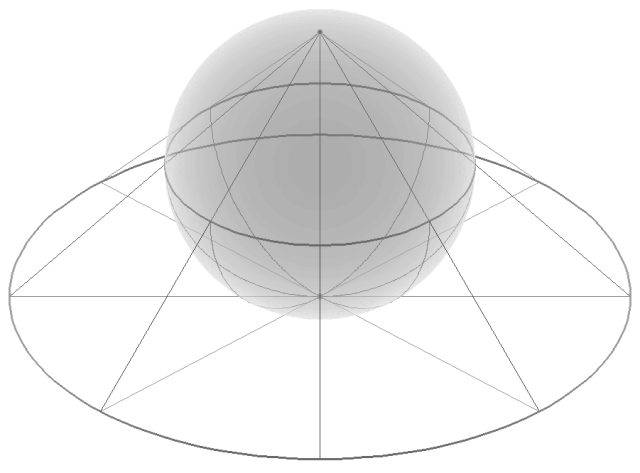
\includegraphics[scale=0.5]{Images/riemannSphere.png}
	\caption{Proyección Estereográfica}
	\label{proy_estereografica}
\end{figure}

Como esta esfera es isomorfa al espacio complejo, existe un isomorfismo entre la esfera y el plano, de modo que todo punto en la esfera tiene asociado un único punto en el espacio complejo.


% CLASE 4
\label{CLASE4}
\subsubsection{Proyección Estereográfica}

Como $\C \cup \{ \infty \} \cong \text{Esfera de Riemann}$, entonces existe un isomorfismo entre ambos espacios. Entonces, a cada punto de la esfera $x_1 ^2 + x_2 ^2 + x_3 ^2 = 1$, se le asocia $z = \flatfrac{(x_1 + ix_2)}{(1 - x_3)}$, es decir: dado $(x_1,x_2,x_3) \in \text{Esfera de Riemann}$
	$$(x_1,x_2,x_3) \mapsto \frac{x_1 + ix_2}{1 - x_3}$$
Para demostrar que dicha transformación es invertible, tomamos el módulo de la parte izquierda:
	$$\abs{z} ^2 = \frac{x_1 ^2 + x_2 ^2}{(1 - x_3)^2}$$
Como dicho punto pertenece a la esfera, entonces se tiene:
	$$ = \frac{1 - x_3 ^2}{(1 - x_3)^2} = \frac{1 + x_3}{1 - x_3}$$
Despejando $x_3$, se tiene:
	$$x_3 = \frac{\abs{z} ^2 - 1}{\abs{z} ^2 + 1}$$
Similarmente, se pueden encontrar expresiones para $x_1$ y $x_2$, con lo que se demuestra que es invertible. Geométricamente, al mapear un punto en la esfera, este punto pertenecerá al plano complejo y a la recta generada por el punto superior de la esfera y el punto de la esfera deseado a mapear.

\paragraph{Ejemplo: } Demostrar que todas las raíces de $p(z) = z^3 + 3z + 5$ tienen módulo mayor a $1$.

\begin{proof}
	Suponiendo que una raíz tiene módulo $\abs{z} \leq 1$, entonces $z^3 + 3z + 5 = 0$, despejando $5$ y enconetrando el módulo de ello se tiene: $\abs{5} = \abs{z^3 + 3z}$ por desigualdad triangular $\abs{z^3 + 3z} \leq \abs{z} ^3 + 3\abs{z}$, por la suposición inicial $\leq 1^3 + 3(1) \leq 4$, lo que es una contradicción, por lo que $\abs{z} > 1$.
\end{proof}
	


% CLASE 5 y 6
\label{CLASE5y6}
\subsection{Teorema de DeMoivre}

Utilizando la notación Eulereana para dos complejos $z,w$, con argumentos $\theta ,\alpha$. Con esto se tiene:
	$$z = \abs{z} e^{i\theta} \quad \quad w = \abs{w} e^{i\alpha}$$
Multiplicando ambos:
	$$zw = \abs{z} \abs{w} e^{i(\theta + \alpha)}$$
Con esta idea, se calcula:
	$$z^n = \abs{z} ^n e^{in\theta}$$
A esto se le conoce como el \textbf{Teorema de DeMoivre}, el cual es cierto, no solo para enteros, sino que para todos los complejos, i.e. $n\in \C$. Esto implica que:
	$$z^n = \abs{z}^n \qty(\cos{n\theta} + i\sin{n\theta})$$

\subsection{Geometría Analítica en $\C$}

\subsubsection{Circunferencia}

Se define como el siguente conjunto:
	$$A = \{ z\in \C : \abs{z} = 1 \}$$
Sin embargo, para una circunferencia desplazada a $z_o$ con radio $r$, se tiene:
	$$\abs{z - z_o} = r$$

\subsubsection{Elipse}

La elipse, asi como en su definición clásica, para sus focos en los puntos $a$ y $b$, se tiene:

	$$\abs{z - a} + \abs{z - b} = k$$
Donde $z$ es todo punto sobre la elipse.

\subsubsection{Recta}

Para una recta entre dos complejos, se tiene que, tomando un parametro $t\in \R$, la recta que pasa por ambos complejos esta dada por:
	$$z + t(z + w)$$
Segmentando dicha recta, se tiene que, para la distancia entre ambos complejos, se limita $t$  a $0 \leq t \leq 1$. Y en base a esto se puede calcular el punto medio entre dos complejos, el cual es simplemente haciendo el valor de $t = 2$.

\subsubsection{Gravicentro}

Sabiendo la relación de las medianas y el gravicentro, entonces tomando los segmentos de recta, simplemente se realiza dicho procedimiento. Tomando cualquier lado (en este caso se tomará $ac$) se tiene que el punto medio entre dichos vértices es:
	$$\frac{a + c}{2}$$
Ahora, para el segmento entre este nuevo punto y el vértice restante es:
	$$b + t\qty(\frac{a + c}{2} - b)$$
Por la relación se tiene que $t = \flatfrac{2}{3}$, con esto y desarrollando se tiene:
	$$\boxed{G = \frac{a + b + c}{3}}$$
	
\dsnote{Ejemplo tarea: \textit{Demostrar que: } $\tan ^2 {1} + \cdots + \tan ^2 {89} \, \in \, \Z$.}



% CLASE 7
\label{CLASE7}
\textbf{Resolviendo el ejemplo: } \\

Tomando la forma polar de un complejo de módulo $1$, se eleva a la $90$ potencia:
	$$\qty(\cos{\alpha} + i\sin{\alpha})^{90} = \cos{90\alpha} + i\sin{90\alpha}$$
Por teorema del Binomio:
	$$\sum _{k=0} ^{90} \binom{90}{k} \cos ^{n - k} {\alpha} \, i^k \sin ^k {\alpha} = \cos{90\alpha} + i\sin{90\alpha}$$
Sabiendo que para potencias pares, la identidad imaginaria es real, entonces:
	$$\sum _{k=0} ^{44} (-1)^k \binom{90}{2k} \cos ^{90 - 2k} {\alpha} \sin ^{2k} {\alpha} = \cos{90\alpha}$$
Reescribiendo el lado izquierdo de la ecuación.

Para $\alpha$ impar:
	$$\sum_{k=0} ^{44} \binom{90}{2k} (-1)^k \tan ^{2k} {\alpha} = 0$$
Entonces, sustituyendo $x = \tan ^2 {\alpha}$, por Cardano$-$Vieta, la suma de todas las soluciones da como resultado uno de los coeficientes del polinomio, por ende, la suma propuesta da como resultado un número entero, por lo que queda demostrado. $\QED$




\section{Funciones Complejas}
Una función compleja, se define igual que las funciones reales, simplemente se tiene que el dominio y el rango son los complejos, es decir:
	$$f:\, \C \to \C$$
En las funciones complejas, no se tienen gráficas como las que se tienen en funciones de $\R$ o $\R^2$. En los complejos, se sabe de, álgebra lineal, que, los complejos son un espacio vectorial de dimensión dos, sobre los reales; de modo que, las funciones son una aplicación de dimension $4$, por lo que no se puede visualizar una gráfica. Para graficar las funciones complejas se toman dos espacios complejos, simplemente para comparar el dominio de la función, con el rango de la misma.

\subsection{Función Exponencial}

Sea $z = x + iy$, se define la exponencial:
	$$e^z := e^x e^{iy}$$
La cual es completamente intuitiva.
	


% CLASE 8
\label{CLASE8}

\subsection{Funciones Seno y Coseno}

Para definir al seno y al coseno, tomamos una forma exponencial:
	$$\sin{z} := \frac{e^{iz} - e^{-iz}}{2i}$$
Y
	$$\cos{z} := \frac{e^{iz} + e^{-iz}}{2}$$

Para la identidad pitagórica, se sabe que se cumple para todo número real; sin embargo, con estas nuevas definiciones, se tiene que dicha identidad es cierta para todo $z\in \C$.

\begin{teorema} \it
	$$\sin ^2 {z} + \cos ^2 {z} = 1$$
\end{teorema}

La demostración es bastante simple, solo se elevan ambas definiciones al cuadrado y por productos notables queda. \\

Además, cumplen todas las identidades ya conocidas para los números reales.
\begin{teorema} \it
	La función:
		$$f(z) = e^{z}$$
	Es periódica, con periodo $2\pi i$
\end{teorema}

Lo curioso de esto, es que la función exponencial para valores reales \textbf{no} es periódica, pero en los complejos si lo es. Para veríficar que la función es periódica simplemente se sustituye la definción de funciones periódicas:
	$$f(z) = f(z + T)$$
La demostración es igual de simple que la anterior, simplemente sustituyendo la definción, se tiene la periodicidad.

\subsubsection{Funciones Seno y Coseno Hiperbólicos}

Para las funciones hiperbólicas, se tienen definiciones muy parecidas a sus respectivas funciones no hiperbólicas, es decir:
	$$\sinh{z} := \frac{e^z - e^{-z}}{2}$$
Y
	$$\cosh{z} := \frac{e^z + e^{-z}}{2}$$
Para todo $z\in \C$.

\subsection{Función Logarítmica}

La función logarítmica debe cumplir ser la inversa de la exponencial, obviamente, en dominio complejo. Entonces, para $z\in \C$, se tiene:
	$$\ln{z} := \ln{\abs{z}} + i\text{arg} (x)$$
Para comprobar que la función logarítmica compleja es, efectivamente, la función inversa de la exponencial. Comprobando con:
	$$f(f^{-1}) = z \quad \quad f^{-1} (f) = z$$
Comprobando que la definción cumple, se tiene:
	$$e^{\ln{z}} = e^{\ln{\abs{z}}} e^{i\text{arg} (z)} = z$$
Ahora, para la otra propiedad de las funciones inversas:
	$$\ln{e^z} = \ln{\abs{e^z}} + i\text{arg} (e^z)$$
Por la forma de la exponencial compleja, se tiene:
	$$= \ln{e^x} + iy = x + iy = z$$
Lo que comprueba las propiedades de función inversa. Cabe recalcar que el logaritmo es una función multivaluada, por lo que se define le logaritmo principal, el cual toma como argumento el argumento principal del complejo. Además, con todo esto, permite encontrar el logaritmo para números negativos. De todo esto, la función logarítmica es válida para $f:\C \setminus \{ 0 \} \to \C$.


% CLASE 9
\label{CLASE9}
\section{Fórmula de Euler}
Tomando $\cos{z} + i\sin{z}$ con $z\in \C$, sustituyendolo por su definición exponencial.
	$$\cos{z} + i\sin{z} = \frac{e^{iz} + e^{-iz}}{2} + i\frac{e^{iz} - e^{-iz}}{2i}$$
Reduciendo, se tiene que:
	$$e^{iz} = \cos{z} + i\sin{z}$$
Para $z\in \C$, esta es la famosa \textbf{Fórmula de Euler}.



% CLASE 10
\label{CLASE10}
\section{Espacios Métricos (Topología de Números Complejos)}

La idea principal de los espacios métricos es la posibilidad de medir distancias.

\begin{definicion} \slshape
	Una función $d:E\times E \to \R$ es una métrica si:
		\begin{enumerate}[a)]
			\item $d(x,y) \geq 0$, para todo $x,y \in E$.
			\item $d(x,y) = 0 \, \Leftrightarrow \, x=y$
			\item $d(x,y) = d(y,x)$ para todo $x,y  \in E$
			\item $d(x,y) \leq d(x,z) + d(z,y)$ para todo $x,y,z\in E$
		\end{enumerate}
\end{definicion}

Si $d:E\times E \to \R$ es una métrica, entonces $(E,d)$ es un espacio métrico. Por ejemplo: 

\begin{itemize}
	\item Tomando $E = \C$ con la métrica definida por el módulo $d(x,y) = \abs{x - y}$, $x,y \in \C$.
	\item Se tiene $E = \C$, para dos elementos del espacio:
		$$d(x,y) = \left\{\begin{array}{cc}
			0 & \text{si } x = y \\
			1 & \text{si } x \neq y
		\end{array}\right.$$
\end{itemize}

\subsection{Proyección Estereográfica}
Tomando un punto en el plano complejo y su respectivo punto en la Esfera de Riemann, la distancia entre dichos dos puntos es:
	$$d(z,z') = \frac{2\abs{z - z'}}{\sqrt{\qty(1 + \abs{z} ^2) \qty(1 + \abs{z'}^2)}}$$
Donde $z$ es el punto en la esfera y $z'$ es el punto sobre el plano complejo.


% CLASE11
\label{CLASE11}
\subsection{Conjuntos Abiertos y Cerrados}

Para iniciar con las definiciones asociadas a ciertos conceptos topológicos, es necesario la base de dichos conceptos, vease, la vecindad, bola, etc. La vecindad se define como:

\begin{definicion} \slshape
	Sea $(E,d)$ un espacio métrico una \textbf{vecindad} centrada en $z_o$ de radio $r>0$ es:
		$$B_r (z_o) := \{ z\in E: d(z_o,z) < r \}$$
	Además, $B$ es vecindad de $w$ si existe $B_r (z_o)$ tal que:
		$$B_r (z_o) \subseteq B$$
\end{definicion}

Con esto, se define:
\begin{definicion} \slshape
	Un conjunto C es \textbf{abierto} si es vecindad de cada uno de sus puntos.
\end{definicion}

\begin{definicion} \slshape
	Un conjunto $C$ es \textbf{cerrado} si $C^c$ es abierto.
\end{definicion}

La definición de conjunto cerrado aparenta ser trivial, sin embargo, la "afirmación": «Un conjunto no es abierto, entonces es cerrado». Puesto que hay conjuntos que son tanto abiertos como cerrados y conjuntos que no son, ni abiertos ni cerrados.



% CLASE12
\label{CLASE12}
\subsection{Sucesiones}

\begin{definicion} \slshape
	Una \textbf{sucesión} de números complejos es una función $f:\N \to \C$. Generalmente representadas como $x_n,(x_n),\ldots$.
\end{definicion}

Ya que se definieron las sucesiones, es lógico pensar en que ciertas sucesiones tienden a ciertos valores, a esto le llamaremos convergencia.

\begin{definicion} \slshape
	Una sucesión $x_n$ \textbf{converge} a un punto $p$ si para cada $\varepsilon > 0$ existe un $N \in \N$ tal que:
		$$d(x_m ,p) < \varepsilon$$
	Si $m > N$.
\end{definicion}

Esta idea induce el siguiente teorema:

\begin{teorema} \it
	Si $x_n$ es convergente, entonces su límite es único
\end{teorema}

\begin{proof}
	Supongamos que $x_n \to p$ y $x_n \to q$. Como $x_n$ convergue a $p$, entonces $\forall \, \varepsilon > 0$ existe $N_1$ tal que:
		$$d(x_m,p) < \frac{\varepsilon}{2} \quad \quad m > N_1$$
	De igual forma, como $x_n \to q$, entonces para todo $\varepsilon > 0$ existe $N_2$ tal que:
		$$d(x_m,q) < \frac{\varepsilon}{2} \quad \quad m > N_2$$
	Por desigualdad triangular
		$$d(p,q) \leq d(x_m ,p) + d(x_m ,q) < \varepsilon \quad \quad \text{si } m > \text{max} \{N_1,N_2 \}$$
	Como se debe de cumplir para todo $\varepsilon > 0$, entonces se tiene $d(p ,q) = 0$ y por definición de métrica se concluye que $p = q$.
\end{proof}

Un teorema más específico para el espacio de los complejos:	

\begin{teorema} \it
	Una sucesión $z_n$ converge a $z = a + bi$ si y solo si
		$$\Re{z_n} \to a$$
	Y
		$$\Im{z_n} \to b$$
\end{teorema}

\dsnote{Se convierte una sucesión de complejos a dos sucesiones independientes de números reales.}


% CLASE 13
\label{CLASE13}
\section{Analiticidad}

\begin{definicion} \slshape
	Una función $f$ es \textbf{derivable} en $z_o \in \C$ si:
		$$\lim _{z\to z_o} \frac{f(z) - f(z_o)}{z - z_o}$$
	existe.
\end{definicion}


\begin{definicion} \slshape
	Una función es \textbf{holomorfa} (analítica) en $z_o$ si es derivable en un abierto que contiene a $z_o$.
\end{definicion}

Al hablar de funciones analíticas recuerda a la definción asociada a series de Taylor, sin embargo, el hecho de que una función compleja es holomorfa, implica directamente que la función sea analítica.

\subsection{Propiedades de las Funciones Holomorfas}
\subsubsection{Teorema de Cauchy$-$Riemann}
\begin{teorema} \it
	Sea $f:\C \to \C$, tal que $f(z) = u(x,y) + iv(x,y)$, donde $z = x + iy$. Entonces si $f$ es holomorfa en $z_o = x_o + iy_o$, entonces
		$$\pdv{x} u(x_o ,y_o) = \pdv{y} v(x_o ,y_o)$$
		$$\pdv{y} u(x_o, y_o) = -\pdv{x} v(x_o ,y_o)$$
	además, $f'(z_o) = u_x (x_o ,y_o) + iv_x (x_o ,y_o)$.
\end{teorema}

Para el converso, si se cumplen las ecuaciones de Cauchy$-$Riemann y las derivadas parciales son continuas, entonces $f$ es holomorfa.

\dsnote{La demostración viene después.}

\begin{ejemplo} \tt
	Demostrar que $f(z) = z^2$ es holomorfa en todos lados y calcular su derivada. \\
	Tomando la función y sustiuyendo $z = x + iy$,
		$$f(z) = (x + iy)^2 = \underbrace{x^2 - y^2}_{u(x,y)} + \underbrace{2xy}_{v(x,y)} i$$
	Es claro que se cumplen las ecuaciones de Cauchy$-$Riemann, además, como las derivadas parciales son continuas para todo $x,y \in \R$, entonces, por el converso del teorema de Cauchy$-$Riemann, la función $f$ es holomorfa. Y la derivada es:
		$$f'(z) = 2x + 2yi = 2z$$
\end{ejemplo}

\begin{definicion} \slshape
	Una función que es holomorfa en todo $\C$ se dice que es \textbf{entera}.
\end{definicion}

\begin{ejemplo} \tt
	Demostrar que $f(z) = e^z$ es entera y calcular su derivada. \\
	
	Separando en parte imaginaria y real:	
		$$f(z) = e^x (\cos{y} + i\sin{y})$$
	En lo que claramente se cumple Cauchy$-$Riemann, y como dichas funciones son continuas en todos los puntos, por lo que, la función es entera. Entonces, la derivada es:
		$$f'(z) = e^x (\cos{y} + i\sin{y}) = e^z$$
\end{ejemplo}

\begin{ejemplo} \tt
	Demostrar que $f(z) = \bar{z}$ no es holomorfa en ningún lado. \\
	Realizando Cauchy$-$Riemann, no se cumple la primera encuación $C-R$. Entonces no es holomorfa en ningún lado. Por lo que dicha función no es derivable.
\end{ejemplo}


% CLASE 15
\label{CLASE15}
\subsubsection{Teorema de la Función Inversa Versión Compleja}
\begin{teorema} \it
	Si $f$ es holomorfa y $f'(z_o) \neq 0$, entonces existe un abierto que contiene a $z_o$ tal que
		$$\dv{w} f^{-1} (w) = \frac{1}{f'(z)}$$
	en donde $w=f(z)$, para $z$ en el abierto.
\end{teorema}

\begin{ejemplo} \tt
	Si $f$ es una función holomorfa, entonces las curvas de nivel de sus partes real e imaginaria son perpendiculares entre si. \\
	Por definición de gradiente, se tiene que:
		$$\langle \grad{u} ,\grad{v} \rangle = u_x v_x + u_y v_y$$
	Por Cauchy$-$Riemann, entonces:
		$$\langle \grad{u} ,\grad{v} \rangle = 0$$
	Lo que los gradientes, se intersectan perpendicularmente, entonces las curvas de nivel se intersectan perpendicularmente. $\QED$
\end{ejemplo}


% CLASE 16
\label{CLASE16}
\subsubsection{Funciones Armónicas}

\begin{definicion} \slshape
	Una función $\phi :\R ^2 \to \R$ es \textbf{armónica} si
		$$\nabla ^2 \phi = 0$$
\end{definicion}



\begin{teorema} \it
	Las partes real e imaginaria de una función holomorfa son armónicas.
\end{teorema}

\begin{proof}
	Sean $f(z) = u(x,y) + iv(x,y)$ una función holomorfa. Entonces, satisface las ecuaciones de Cauchu$-$Riemann:
		$$u_x = v_y \quad \quad u_y = - v_x$$
	Derivando otra vez las ecuaciones de C$-$R y, utilizando el teorema de Cairaut, derivando respecto a $x$, se tiene:
		$$u_{xx} + u_{yy} = v_{xy} - v_{yx} = 0$$
	Similarmente, $v$ es armónica.
\end{proof}


\begin{definicion} \slshape
	Sea $u$ una función armónica. Una función $v: \R^2 \to \R$ que hace que la función:
		$$f(z) = u + iv$$
	sea holomorfa, se le llama \textbf{Conjugado Armónico} de $u$.
\end{definicion}



\subsection{Demostración Teorema Cauchy$-$Riemann}
Tomando la definición compleja de derivada:
	$$f'(z_o) = \lim_{\Delta z \to 0} \frac{f(z_o + \Delta z) - f(z_o)}{\Delta z}$$
Sabiendo que para determinar la existencia de un límite de una función compleja (siguiendo la idea del calculo multivariable), es necesario que desde cualquier trayectoria, hacia el punto en concreto el límite tenga el mismo valor. Por lo que, reescribiendo el límite:
	$$ = \lim _{\Delta z \to 0} = \frac{u(x_o + \Delta x, y_o + \Delta y) + iv(x_o + \Delta x, y_o + \Delta y) - u(x_o,y_o) - v(x_o,y_o)}{\Delta x +i\Delta y}$$
	
Tomando dos formas para aproximarse al cero, de este nuevo límite, es, primero, aproximando por el eje real.
	
	$$ = \lim _{\Delta x \to 0} \frac{u(x_o + \Delta x, y_o) - u(x_o,y_o)}{\Delta x} + i\lim _{\Delta x \to 0} \frac{v(x_o + \Delta x, y_o) - v(x_o,y_o)}{\Delta x} = \pdv{u}{x} (x_o,y_o) + i\pdv{v}{x} (x_o,y_o)$$
La segunda forma, es por medio del eje imaginario:
	$$\lim _{\Delta y \to 0} \frac{u(x_o, y_o + \Delta y) - u(x_o,y_o)}{i\Delta y} + i\lim _{\Delta x \to 0} \frac{v(x_o, y_o + \Delta y) - v(x_o,y_o)}{i\Delta y} = -i\pdv{u}{y} (x_o,y_o) + \pdv{v}{y} (x_o,y_o)$$

Como $f'(z_o)$ existe, se sabe que todoslos caminos diferentes para aproximar $\Delta z\to 0$ deben ser iguales; de modo que, igualando parte real y parte imaginaria se tiene:
	$$\pdv{u}{x} = \pdv{v}{y} \quad \quad \pdv{u}{y} = -\pdv{v}{x}$$
$\QED$

% CLASE 14
\label{CLASE14}
\section{Límites en Funciones Complejas}

Se define límite para una función definida de $f:\C \to \C$:

\begin{definicion} \slshape
	Sea $f$ definida en un conjunto que contiene alguna vecindad de radio $r$ centrada en $z_o$. Se dice que el límite cuando $z$ tiende a $z_o$ de $f(z)$ es $w$, el cual se denota por:
		$$\lim _{z\to z_o} f(z) = w$$
	si para cada $\varepsilon > 0$, existe $\delta > 0$ tal que para todo $z\neq z_o$ en $V_r (z_o)$, se cumple que
		$$\abs{f(z) - w} < \varepsilon$$
	Siempre que $\abs{z - z_o} < \delta$.
\end{definicion}

\begin{teorema} \it
	El límite de una función compleja es \textbf{único}, si es que existe.
\end{teorema}

\begin{proof}
	Supongamos que:
		$$\lim _{z\to z_o} f(z) = a$$
	Y 
		$$\lim _{z\to z_o} f(z) = b$$
	con $a\neq b$ y, sea $\varepsilon = \flatfrac{\abs{a - b}}{2} > 0$. Por definición de límite, sea $\delta > 0$ tal que $\abs{z - z_o} <\delta$ implica que $\abs{f(z) - a} < \varepsilon$ y $\abs{f(z) - b} < \varepsilon$.
	Entonces:
		$$\abs{a - b} \leq \abs{a - f(z)} + \abs{f(z) - b} < 2\varepsilon$$
	Lo que claramente es una contradicción, entonces $a\neq b$.
\end{proof}

Lo interesante es que para funciones de variable compleja, las propiedades de los límites (álgebra de los límites) sigue siendo igual, por lo que no se ahondará en ello.

\begin{ejemplo} \tt
	Determinar si el límite existe:
		$$\lim _{z\to 0} \qty(\frac{z}{\bar{z}}) ^2$$
	Como en varias variables, para que un límite exista, es necesario que de el mismo valor desde todas sus trayectorias, por lo que, es más sencillo determinar la no existencia del límite; de modo que, acercandolos por la trayectoria sobre el eje real:
		$$\lim _{z\to 0} \qty(\frac{x}{x})^2 = 1$$
	Y por la recta $y=x$:
		$$\lim _{z\to 0} \qty(\frac{x + xi}{x - xi}) ^2$$
	Luego de un poco de desarrollo algebraico, se tiene que dicho límite es igual a:
		$$\lim _{z\to 0} \qty(\frac{x + xi}{x - xi}) ^2 = e^{i\pi} = -1$$
	Por lo que el límite no existe.
\end{ejemplo}

\subsection{Continuidad}

\begin{definicion} \slshape
	Una funcion compleja $f$ es continua en $z_o$ si su límite existe y:
		$$\lim _{z\to z_o} f(z) = f(z_o)$$
\end{definicion}






\dsnote{Lo siguiente no esta ordenado en relación a temas, aun.}

\begin{definicion} \slshape
	Una función $\phi :\R ^2 \to \R$ es \textbf{armónica} si
		$$\nabla ^2 \phi = 0$$
\end{definicion}



\begin{teorema} \it
	Las partes real e imaginaria de una función holomorfa son armónicas.
\end{teorema}

\begin{proof}
	Sean $f(z) = u(x,y) + iv(x,y)$ una función holomorfa. Entonces, satisface las ecuaciones de Cauchu$-$Riemann:
		$$u_x = v_y \quad \quad u_y = - v_x$$
	Derivando otra vez las ecuaciones de C$-$R y, utilizando el teorema de Cairaut, derivando respecto a $x$, se tiene:
		$$u_{xx} + u_{yy} = v_{xy} - v_{yx} = 0$$
	Similarmente, $v$ es armónica.
\end{proof}



\begin{lema} \it
	Si $f$ es una función diferenciable en $z_o$, entonces $f$ es continua en $z_o$.
\end{lema}





% CLASE15
\label{CLASE15}
\section{Mapeos}

Ejemplo función $f(z) = z^2$, aplicada a 

\begin{ejemplo} \tt
	Para la función $f(z) = z^2$ aplicada a las rectas $1 + yi$ y $x + i$ se tiene que.
		$$(1 - y^2) + 2yi$$
		$$\color{red} (1 - y^2) + 2yi$$
	Las cuales son las ecuaciones paramétricas de dos parábolas en sistemas ortogonales $u$ y $v$. Otra cosa curiosa a notar es la conservación del ángulo entre las curvas, como se ve en la figura \ref{Parabolas}
	\begin{figure}[H]
		\centering
		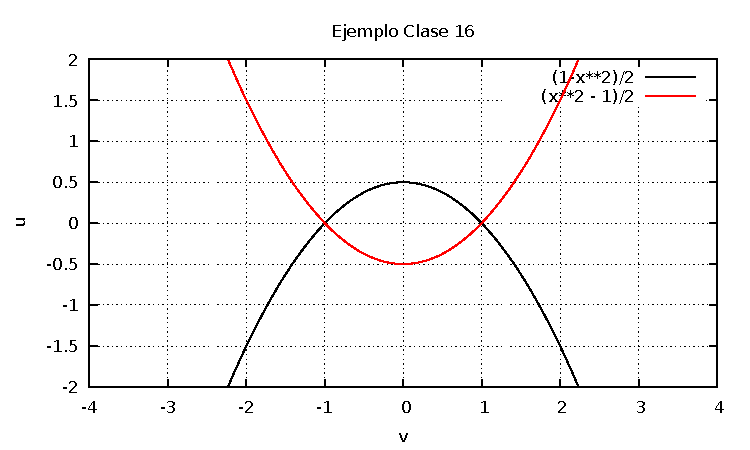
\includegraphics[scale=1.2]{Images/Parabolas.pdf}
		\caption{Parabolas en el Sistema $v,u$}
		\label{Parabolas}
	\end{figure}
	En la cual es claro ver que las parábolas se intersectan a un ángulo de $90^o$.
\end{ejemplo}




\begin{ejemplo} \tt
	Tomando las rectas $1 + iy$ y $x + i$, las cuales son claramente perpendiculares. Para el mapeo $f(z) = e^z$, se tienen las siguientes dos curvas
		$$ee^{iy} \quad \quad \quad \quad e^x e^i$$
	De las cuales la primera es un círculo de radio $e$, y la segunda es una recta con una pendiente de $1rad$. Como la recta sale del centro y la circunferencia esta centrada en el $0$, entonces el ángulo entre la circunferencia y la recta también es de $90^o$.
\end{ejemplo}



\subsection{Repaso Cálculo Multivariable}


\begin{definicion} \slshape
	Dada una curva $C$ por las ecuaciones paramétricas 
		$$\left\{\begin{array}{c}
			x = f(t) \\
			y = g(t)		
		\end{array}\right.
		$$
	en un intervalo cualquiera, es \textbf{suave} si sus derivadas son continuas en el intervalo y no son simultaneamente nulas (todos los puntos que no sean singulares), excepto posiblemente en los puntos terminales del intervalo.
\end{definicion}

Luego de esto es lógico preguntarse como determinar si una curva es singular en algún punto. De esto, se define singularidad:
\begin{definicion} \slshape
	Sea $(x(t),y(t))$ una curva plana. Decimos que es \textbf{singular} en $(x(t_o),y(t_o))$ si
		$$(\dot{x}(t_o),\dot{y}(t_o)) = (0,0).$$
	Una curva es suave en todos sus puntos sino es singular.		
\end{definicion}



\subsection{Mapeos Conformes}

\begin{definicion} \slshape
	\textbf{Mapeos Conformes}
	Sea $w = f(w)$ un mapeo coplejo definido en un abierto conexo $D$ y sea $z_o \in D$. Entonces decimos que $w=f(z)$ es \textbf{conforme} en $z_o$ si para todo par de curvas suaves $C_1$ y $C_2$ que se interesectan en $z_o$ el ángulo entre $C_1$ y $C_2$ es igual al ángulo entre $f(C_1)$ y $f(C_2)$ en magnitud y sentido.
\end{definicion}

% CLASE 18
\label{CLASE18}

Una forma más directa para determinar si un mapeo es conforme es por medio del siguiente teorema, el cual enlaza con el concepto de función holomorfa

\begin{teorema} \it
	Si $f$ es holomorfa en un abierto conexo $D$ que contiene a $z_o$, y si $f' (z_o) \neq 0$, entonces $w = f(z)$ es conforme en $z_o$.
\end{teorema}

Esto se puede ver claramente con el ejemplo del mapeo $f(z) = e^z$.

\begin{proof}
	Tomando dos curvas suaves $z_1$ y $z_2$ que se intersectan en $z_o$ se tiene que el ángulo entre dichas curvas en $z_o$ está dado por
		$$\theta = arg(z' _1 (z_o)) - arg(z' _2 (z_o))$$
	Con esta idea, se toma el mapeo $f$ de modo que
		$$w_1 = f(z_1)$$
		$$w_2 = f(z_2)$$
	El ángulo $\hat{\theta}$ entre $w_1$ y $w_2$ en $f(z_o)$ es:
		$$\hat{\theta} = arg\qty(w' _1 (f(z_o))) - arg\qty(w' _2 (f(z_o)))$$
	Por regla de la cadena
		$$ = arg\qty(f'(z_o) z' _1 (z_o)) - arg\qty(f'(z_o) z' _2 (z_o))$$
	Sabiendo que el argumento del producto es la suma de los argumentos (esto se puede ver claramente con la notación Euleriana de los complejos), se tiene
		$$\hat{\theta} = arg(z' _1 (z_o)) - arg(z' _2 (z_o)) = \theta$$
\end{proof}

Para introducir mejor el siguiente teorema, se puede tomar el mapeo $f(z) = z^2$ el cual es una función holomorfa y, conforme en $z \neq 0$. Aplicando el mapeo a $z_1 = x$ y $z_2 = yi$, se tiene que las imagenes de ambas curvas son los reales positivos y negativos, respectivamente. Con lo que es claro que el ángulo se duplica, con esta idea, el siguiente teorema es más claro: \\

\begin{teorema} \it
	Sea $f$ una función holomorfa en un abierto conexo $D$ que contiene a $z_o$ y $f'(z_o) = 0$. Si $n > 1$ es un entero tal que
		$$f'(z_o) = f''(z_o) = f'''(z_o) = \cdots = f^{(n - 1)} (z_o) = 0$$
	Pero $f^{(n)} (z_o) \neq 0$ entonces el ángulo entre cualesquiera dos curvas suaves que se intersectan en $z_o$ aumenta en un factor de $n$, por el mapeo $w = f(z)$.
\end{teorema}





% CLASE 19
\label{CLASE19}
\section{Integración Compleja}

Muy parecido a como se realiza en el campo $\R$, se realizan las integrales en los complejos. Sea $h: [a,b] \subset \R \to \C$ una función compleja con $u$ y $v$ como su parte real y parte imaginaria, respectivamente. Se define la integral sobre $[a,b]$ como: $t\in \R$
	$$\int _a ^b h(t) \dd{t} = \int _a ^b u(t) \dd{t} + i\int _a ^b v(t) \dd{t}$$ 
	
Además para una curva parametrizada como $c:z(t)$, se tiene que la integral de una función compleja sobre dicha curva, es	
	$$\int _c f(z) \dd{z} = \int f(z(t)) \dot{z}(t) \dd{t}$$
	
\subsection{Integrales sobre Curvas}

Sea $\alpha (t)$ una curva parametrizada como $z(t) = x(t) + iy(t)$ con $a\leq t \leq b$, entonces
	$$\int _\alpha f(z) \dd{z} = \int _a ^b f(z(t)) z'(t) \dd{t}$$

\begin{ejemplo} \tt
	Calcular $\int_\alpha \frac{1}{z} \dd{z}$, donde $\alpha$ es la curva $\abs{z} = 1$. \\
	Sabiendo que la curva $\abs{z} = 1$ es el circulo unitario, es claro que $z(t) = e^{it}$ con $0 \leq t 2\pi$. Derivando $z'(t) = ie^{it}$. Sustituyendo en la definición se tiene que
		$$\int _{\abs{z} = 1} \frac{1}{z} \dd{z} = 2\pi i$$
\end{ejemplo}



\begin{ejemplo} \tt
	Calcular $\int_\alpha \frac{1}{z^2} \dd{z}$, donde $\alpha$ es la curva $\abs{z} = 1$. \\
	Con esto, se toma la parametrización del circulo unitario $z(t) = e^{it}$, sustituyendo en la definición de integrales sobre la curva se tiene la siguiente integral:
		$$ = \int _0 ^{2\pi} \frac{1}{e^{2it}} ie^{it} \dd{t}$$
	Lo cual, luego de integral, se tiene
		$$ = \eval[-e^{it}|_{0} ^{2\pi} = 0$$
	
\end{ejemplo}


Generalizando estos dos ejemplos, se puede concluir que:
	$$\int _{\abs{z}  =1} \frac{1}{z^n} \dd{z} = 
	\left\{\begin{array}{ccc}
		0 & \text{si} & n > 1 \\
		2\pi i & \text{si} & n = 1
	\end{array}\right.
	$$
Para todo $n\in \N$.



\subsection{Teorema Fundamental}

Suponiendo que $\alpha : [a,b] \to \C$ es una curva suave a trozos que $F$ es una función analítica en un conjunto abierto $G$ que contiene a $\alpha$. Entonces,
	$$\int _\alpha F'(z) \dd{z} = F(\alpha (b)) - F(\alpha (a))$$


\begin{ejemplo} \tt
	Calcular $\int _\alpha z^3 \dd{z}$, donde $\alpha$ es la parte de la elipse $x^2 + 4y^2 = 1$ que una a los puntos $z = 1$ y $z = \frac{i}{2}$. \\
	Sabiendo que
		$$z^3 = \dv{z} \qty(\frac{1}{4} z^4)$$
	Con esto se tiene, por el teorema fundamental
		$$\int _\alpha z^3 \dd{z} = \eval[\frac{1}{4} z^4|_1 ^{\flatfrac{i}{2}} = -\frac{15}{61}$$
\end{ejemplo}



\subsubsection{Teorema de Cauchy$-$Goursat}


\begin{teorema} \it
	Sea $f$ una función holomorfa en un dominio simplemente conexo $A$, entonces para toda curva cerrada simple $\alpha$ en $A$.
		$$\oint _\alpha f(z) \dd{z} = 0$$
\end{teorema}


\begin{proof}
	Descomponiendo la función y la integral en componentes, sabiendo que $f = u + iv$
		$$\int _x f(z) \dd{z} = \int _c (u+iv)(\dd{x} + i\dd{y}) = \int _c u\dd{x} - v\dd{y} + i\int _c v\dd{x} + u\dd{y}$$
	Como las integrales que resultaron son de variable real, se puede utilizar el teorema de Green a cada una de las mismas, de modo que
		$$ = \iint _R (-v_x - u_y) \dd{A} + i\iint _R (u_x - v_y) \dd{A}$$
	Como la función es holomorfa en el interior de $c$ y en su borde, entonces es válido Cauchy$-$Riemann y, por esto, las integrales son cero. Por lo tanto
		$$\int _c f(z) \dd{z} = 0$$
\end{proof}


El trabajo de Goursat en este teorema fue, quitar la condición de que la primera derivada de $f$ fuera continua. Además, con los ejemplos dados al inicio de esta sección, queda claro que el converso del teorema de Cauchy$-$Goursat (como se enunció) no es cierto, al menos no de manera general.





\subsubsection{Fórmulas de Integración de Cauchy}


Como consecuencia inmediata del teorema de Cauchy$-$Goursat se tiene el siguiente teorema.

\begin{teorema} \it
	{\bf Teorema de Deformación} \\
	Sea $f$ holomorfa en una región $A$ y sea $C$ una curva cerrada simple en $A$. Supongamos que $C$ se puede deformar continuamente en $\hat{C}$ sin salir de la región $A$, entonces
		$$\int _C f(z) \dd{z} = \int _{\hat{C}} f(z) \dd{z}$$
	\begin{proof}
		La idea de la demostración es la misma que la demostración del teorema de Green. Sean $C$ y $\hat{C}$ curvas unidas por dos curvas diferentes cercanas $\alpha$ y $\hat{\alpha}$. Con esto, la integral sobre esa curva es
			$$\int _{\hat{C} + \alpha - C + \hat{\alpha}}$$
		Por Cauchy$-$Goursat dicha integral es cero, además, realizando el límite en el cual la separacion entre $\alpha$ y $\hat{\alpha}$ es cero, entonces se tiene:
			$$\int _{\hat{C}} f \dd{z} + \int _{\alpha} f \dd{z} - \int _{C} f \dd{z} - \int _{\alpha} f \dd{z} = 0$$
		Lo que, claramente, impica que
			$$\int _{\hat{C}} f \dd{z} = \int _{C} f \dd{z}$$
	\end{proof}
\end{teorema}


Del teorema de Cauchy$-$Goursat, se pueden crear ciertos casos interesantes.

\begin{teorema} \it
	\textbf{Primera fórmula Integral de Cauchy} \\
	Sea $C$ una curva cerrada simple, $f(z)$ holomorfa en $C$ y en su interior, entonces para cualquier $z_o$ dentro de la curva, se cumple:
	$$\oint _C \frac{f(z)}{(z - z_o)} \dd{z} = 2\pi if(z_o)$$
	\begin{proof}
		Utilizando el teorema de deformación, se transforma la curva $C$ a una nueva curva $\hat{C}$, la cual será un círculo dentro de la región limitada por la curva $C$. Lo que quedaría
			$$ = \int _{\hat{C}} \frac{f(z_o) - f(z_o) + f(z)}{z - z_o} \dd{z} = \int _{\hat{C}} \frac{f(z_o)}{z - z_o} \dd{z} + \int _{\hat{C}} \frac{f(z) - f(z_o)}{z - z_o} \dd{z}$$
		Parametrizando $\hat{C}$ como $\hat{C}:z_o + re^{it}$ ya se sabe que:
			$$ = 2\pi i f(z_o) + \int _{\hat{C}} \frac{f(z) - f(z_o)}{z - z_o} \dd{z}$$
		Como $f$ es holomorfa en $z_o$ entonces, es contínua en $z_o$; es decir, para todo $\varepsilon > 0$ existe $\delta > 0$ tal que
			$$\abs{f(z) - f(z_o)} < \varepsilon \quad \quad \text{si} \quad \quad \abs{z - z_o} < \delta$$
		Con esta idea, tomaremos el radio de la curva como $r = \frac{\delta}{2}$. Entonces se tiene que $\abs{z - z_o} = \frac{\delta}{2} < \delta$. Además, utilizando la desigualdad $ML$ (mostrada más adelante en esta sección), se tiene que $M = \flatfrac{\varepsilon}{\frac{\delta}{2}}$ y $L = 2\pi \frac{\delta}{2}$, lo que implica que
			$$\abs{\int _{\hat{C}} \frac{f(z) - f(z_o)}{z - z_o} \dd{z}} < ML = 2\pi \varepsilon$$
		Lo que claramente implica que el módulo de dicha integral es cero. Lo que concluye la prueba.
	\end{proof}
\end{teorema}

Generalizando esta idea.

\begin{teorema} \it
	\textbf{Segunda fórmula Integral de Cauchy} \\
	Sea $C$ una curva cerrada simple, $f(z)$ holomorfa en $C$ y en su interior, entonces para cualquier $z_o$ dentro de la curva, se cumple:
	$$\oint _C \frac{f(z)}{(z - z_o)^{n+1}} \dd{z} = \frac{2\pi i}{n!}f^{(n)} (z_o)$$
	 \begin{proof}
	 	
	 \end{proof}
\end{teorema}



\subsubsection{Desigualdad $ML$}
La desigualdad $ML$ tiene cierta importancia a nivel puramente teórico, puesto que permite realizar la demostración de ciertos teoremas importantes.


\begin{teorema} \it
	Sea $C$ una curva poligonal, no necesariamente cerrada, de longitud $L$ y sea $f$ una funcion continua en dicha curva (todo sobre $\C$). Si existe un número real $M > 0$ tal que $\abs{f(z)} \leq M$ para todo $z$ en $C$, entonces
	$$\abs{\int _C f(z) \dd{z}} \leq ML$$

\end{teorema}

\begin{proof}
	Parametrizando la curva como usualmente se hace, $z = z(t), \, a\leq t \leq b$, se obtiene, por la integración compleja vista al inicio de esta sección
	$$\abs{\int _C f(z) \dd{z}} = \abs{\int _a ^b f(z(t)) z'(t) \dd{t}}$$
Por propiedades de las integrales (desigualdad triangular)
	$$\leq \int _a ^b \abs{f(z(t))} \abs{z'(t)} \dd{t}$$
Por hipótesis, la cota superior de $f$ es $M$
	$$\leq M \int _a ^b \abs{z'(t)} \dd{t}$$
La cual es la definición de longitud de arco, como se sabe que la curva tiene una longitud $L$, entonces
	$$\leq ML$$
\end{proof}

Ya con esto, para visualizar la utilidad del teorema, realizamos el siguiente ejemplo.



\begin{ejemplo} \tt
	Demostrar que
		$$\abs{\int _C \frac{\dd{z}}{z^2 + 1}} \leq \frac{\pi}{3}$$
	donde $C$ es la parte del círculo $\abs{z} = 2$ en el primer cuadrante. \\
	Sabiendo la desigualdad triangular con signos cambiados ($\abs{z + w} \geq \abs{\abs{z} - \abs{w}}$), se tiene
		$$M:\abs{\frac{1}{z^2 + 1}} \leq \frac{1}{\abs{z}^2 - 1} = \frac{1}{3}$$
	Además, la longitud de la curva, al ser un segmento de circunferencia, es bastante simple de calcular, de modo que $L = \pi$. Ya con esto, se aplica la desigualdad $ML$, entonces
		$$\abs{\int _C \frac{\dd{z}}{z^2 + 1}} \leq \pi \frac{1}{3}$$
	Justo lo que se quería demostrar. $\QED$
\end{ejemplo}




\subsubsection{Desigualdad de Cauchy}

Sea $f$ holomorfa en un dominio simplemente conexo $D$ y $C$ una circunferencia dada por $\abs{z - z_o} = r$, que se encuentra completamente contenida en $D$. Si $\abs{f(z)} \leq M$ para todos los puntos $z$ en $C$, entonces
	$$\abs{f^{(n)} (z_o)} \leq \frac{n! M}{r^n}$$
	
\begin{proof}
	Partiendo de
		$$\abs{\frac{f(z)}{(z - z_o) ^{n + 1}}} \leq \frac{M}{r^{n + 1}}$$
	Entonces, utilizando la segunda fórmula de Cauchy
		$$\abs{f^{(n)} (z_o)} = \abs{\frac{n!}{2\pi i} \oint _C \frac{f(z)}{(z - z_o) ^{n + 1}} \dd{z}}$$
	Utilizando la desigualdad $ML$
		$$\leq \frac{n!}{2\pi} \frac{M}{r^{n + 1}} 2\pi r = \frac{n! M}{r^n}$$
\end{proof}


Como un corolario de esta desigualdad, se deduce el teorema de Liuville.

\begin{teorema} \it
	Las únicas funciones enteras acotadas son constantes.
	\begin{proof}
		Supongamos que $\abs{f(z)} \leq M$. Sea $z_o \in \C$, sea $r$ suficientemente grande (esto es válido dado que la función es entera)
			$$\abs{f'(z_o)} \leq \frac{M}{r^n}$$
		Lo que hace a la cantidad $\flatfrac{M}{r^n} \to 0$, como es para cualquier número complejo, entonces la función $f$ es constante.
	\end{proof}
\end{teorema}


Este teorema es muy importante en varias ramas de la matemática, en especial el álgebra, puesto que permite demostrar el teorema fundamental del álgebra. 


\subsubsection{Teorema Fundamental del Álgebra}

Para demostrar este teorema, se utilizará un teorema auxiliar, el teorema del Módulo Máximo.

\begin{teorema} \it
	Este teorema es enunciado de dos formas equivalentes:
	\begin{itemize}
		\item Si $f(z)$ es una función holomorfa en un conjunto cerrado simplemente conexo $D$, entonces $\abs{f(z)}$ alcanza el valor máximo en la frontera de $D$.
		\item Sea $f(x)$ es una función holomorfa en un conjunto abierto simplemente conexo $D$, si $\abs{f(z)}$ alcanza el máximo en $D$, entonces $f$ es constante.
	\end{itemize}
\end{teorema}




Dado esto, se demostrará el teorema fundamental del álgebra.

\begin{teorema} \it
	Todo polinomio no constante $p(z)$ tiene al menos una raíz.
	\begin{proof}
		Considerando un polinomio
			$$p(z) = a_n z^n + a_{n - 1} z^{n - 1} +\cdots + a_1 z + a_o,$$
		con $n > 0$. Suponiendo que $p(z)$ no tienen ninguna raíz, la función $f(z)$ definida por
			$$f(z) = \frac{1}{p(z)},$$
		la cual es holomorfa en todo $\C$, i.e. es entera. Para comprobar que la función es acotada. Encontrando el módulo
			$$\abs{f(z)} = \frac{1}{\abs{a_n z^n + \cdots + a_1 z + a_o}} = \frac{1}{\abs{z}^n \abs{a_n + (a_{n-1}/z + \cdots + a_1 / z^{n-1} + a_o / z^n)}}.$$
		Sea $M > 1$ tal que
			$$M > \abs{\frac{2na_j}{a_n}},$$
		para $j = 0,\ldots , n - 1$. Reduciendo un poco, se llega a que, si $\abs{z} > M$,
			$$\abs{\frac{a_j}{z^{n - j}}} < \abs{\frac{a_n}{2n}},$$
		por lo que
			$$\abs{a_{n-1}/z + \cdots + a_1 / z^{n-1} + a_o / z^n} \leq \frac{\abs{a_n}}{2}.$$
		Volviendo a la función $f$, se llega a 
			$$\abs{f(z)} \leq \frac{1}{\abs{z}^n \abs{a_n + (a_{n-1}/z + \cdots + a_1 / z^{n-1} + a_o / z^n)}}$$
			$$\leq \frac{1}{M^n \abs{\abs{a_n} - \abs{a_n}/2}} = \frac{2}{M^n \abs{a_n}},$$
		$f$ es acotada en $\abs{z} > M$, utilizando el Teorema de Weierstrass\footnote{Sea $f$ una función continua en un intervalo compacto, entonces la función alcanza un valor máximo y mínimo en el intervalo.}. Esto implica que la función es acotada, por Liouville se concluye que $f$ es constante, por ende $p$ es constante $(\to \leftarrow)$. Por lo que $p$ si tiene alguna raíz.
	\end{proof}
\end{teorema}

Esta demostración al analizarla bien, demuestra que si el polinomio posee una raíz, entonces tiene $n$ raíces. Esto se debe a la factorización que se le da al polinomio generado una expresion del tipo $p(z) = (z - z_1) q(z)$.

\subsubsection{Teorema de Morera}

Se había mencionado que el converso del teorema de Cauchy$-$Goursat no era cierto de manera general. El teorema de Morera no es el converso del teorema de Cauchy$-$Goursat, ni el teorema de Cauchy$-$Goursat es el converso del teorema de Morera.

\begin{teorema} \it
	Si $f$ es continua en un dominio abierto conexo $D$ y si
		$$\oint _C f(z) \dd{z} = 0,$$
	para cada contorno cerrado $C$ en $D$, entonces $f$ es analítica en $D$.
\end{teorema}






\section{Series}

\subsection{Series de Laurent}
Es una especie de generalización con las series de potencias. En variable real se habla del intervalo de convergencia de la serie, en variable compleja se habla de anillo de convergencia. En las series de Laurent contiene no solo los exponentes negativos. \\

Por ejemplo, las series de Lauren se suelen escribir de la siguiente forma
	$$f(z) = \cdots + a_{-1} (z - z_o)^{-1} + a_o + a_1 (z - z_o) + a_2 (z - z_o)^2 + \cdots$$


Lo que implica que, el punto $z_o$ no puede estar incluído el conocido, radio de convergencia, por lo que se le llama anillo de convergencia.



\begin{ejemplo} \tt
	Encontrar la serie de Lauren de 
		$$f(z) = \frac{\sin{z}}{z^3},$$
	en un anillo centrado en $0$. \\
	Sabiendo que la serie de Taylor de la función $\sin{z}$
		$$\sin{z} = z - \frac{z^3}{3!} + \cdots .$$
	Dividiendo entre $z^3$
		$$f(z) = \frac{1}{z^2} - \frac{1}{3!} + \frac{z^2}{5!} \cdots ,$$
	la cual convergue para los mismos valores para los que convergue el $\sin{z}$ excepto el $0$.
\end{ejemplo}



\begin{ejemplo} \tt
	Encontrar la serie de Lauren de 
		$$f(z) = e^{\flatfrac{1}{z}},$$
	en un anillo centrado en $0$. \\
	Se sabe que la serie de Taylor de la exponencial es
		$$e^z = \sum _{n = 0} ^\infty \frac{x^n}{n!}.$$
	Sustituyendo $\flatfrac{1}{z}$
		$$e^{\flatfrac{1}{z}} = 1 + \frac{1}{2} + \frac{1}{2!} \qty(\frac{1}{z}) ^2 + \cdots .$$
	La cual es la serie de Laurent de dicha función, la cual convergue para todo $\C$ excepto el $0$.
\end{ejemplo}

\subsection{Clasificación de Singularidades}

Sea 
$$f(z) = \cdots + a_{-1} (z - z_o)^{-1} + a_o + a_1 (z - z_o) + \cdot ,$$
la serie de Laurent de $f(z)$ en algún anillo $0 < \abs{z - z_o} < R$, y $z_o$ una singularidad de $f$, entonces:

\begin{enumerate}[a)]
	\item $z_o$ es una singularidad removible, si la serie de Laurent no tiene exponentes negativos.
	\item $z_o$ es una singularidad esencial, si la serie de Laurent tiene infinitos términos con exponentes negativos.
	\item $z_o$ es un polo, si la serie de Laurent tiene una cantidad finita de exponentes negativos; además, si $a_{-n}$ es el menor coeficiente no nulo, entonces $z_o$ es un polo de orden $n$.
\end{enumerate}

Para ejemplificar de mejor manera la implicación de la definición dada:

\begin{ejemplo} \tt
	Clasificar las singularidades de
		$$f(z) = e^{\flatfrac{1}{z}}$$
	La singularidad $z_o = 0$, la serie de Laurent para la exponencial esta dada por
		$$e^{\flatfrac{1}{z}} = 1 + \frac{1}{2} + \frac{1}{2!} \qty(\frac{1}{z}) ^2 + \cdots,$$
	lo que implica que $z_o$ es una singularidad esencial.
\end{ejemplo}






\begin{ejemplo} \tt
	Clasificar las singularidades de
		$$f(z) = \frac{\sin{z}}{z}$$
	La singularidad de $f$ esta en $z_o = 0$ y su serie de Laurent es:
		$$f(z) = 1 - \frac{z^2}{3!} + \cdot,$$
	como no hay términos de exponentes negativos, la singularidad removible.
\end{ejemplo}




\begin{ejemplo} \tt
	Clasificar las singularidades de
		$$f(z) = \frac{1}{z(z - 1)}$$
	La singularidades de $f$ estan en $z_o = 0$ y $z_o = 1$. Para ver que tipo de singularidades son, es necesario encontrar una serie de Laurent. Reescribiendo la función
		$$f(z) = \frac{-1}{z} \qty(\frac{1}{1 - z}),$$
	por la serie geométrica
		$$1 + z + z^2 + \cdots = \frac{1}{1 - z}.$$
	Sustituyendo en la función
		$$f(z) = -\frac{1}{z} - 1 - z - z^2 - \cdots,$$
	por ende, $z_o = 0$ es un polo de orden $1$. Para $z_o = 1$ manipulando la función para generar la serie de Laurent
		$$f(z) = \qty(\frac{1}{z - 1}) \qty(\frac{1}{1 + (z - 1)}),$$
	utlizando la serie geométrica con $x = -(z - 1)$; de modo que
		$$f(z) = \qty(\frac{1}{(z - 1)}) \qty[1 - (z - 1) + (z - 1)^2 - \cdots] = \frac{1}{z - 1} - 1 + (z - 1) - (z - 1)^2 + \cdots,$$
	por lo que $z_o = 1$ es un polo de orden $1$.
\end{ejemplo}











































